\documentclass[a4paper,10pt]{article}

\usepackage[utf8]{inputenc}
\usepackage[T1]{fontenc}
\usepackage[french]{babel}
\AutoSpaceBeforeFDP

\usepackage{amsthm, amsmath,amsfonts, amssymb, latexsym}
\usepackage{color,graphicx,psfrag}
\usepackage{verbatim}
\usepackage{mathpazo}
\usepackage{url}
\usepackage{palatino}

\usepackage{fullpage}

\newcommand{\note}[1]{\textit{\textcolor{blue}{#1}}}

\newcommand{\titlegame}[1]{\subsubsection*{\begin{center}#1\end{center}}}

\usepackage{listings}
\lstdefinelanguage{GameGrammar}{
  morekeywords=[1]{type,is,has,multiple,enemy,ally,neutral,player,game,at,in,on,list,of,with,means,desactivate,activate,definition,command,rule,then},
  morekeywords=[2]{Object,Character}
}

\newcommand{\code}[1]{
\lstset{
  language=GameGrammar,
  basicstyle=\scriptsize\ttfamily,
  commentstyle=\color{blue},
  keywordstyle=[1]\bfseries,
  keywordstyle=[2]\itshape
}
\lstinline{#1}}

\lstnewenvironment{GameGrammar}[1][]{\lstset{language=GameGrammar}#1}{}



\title{Plateforme de création de "mini" jeux 3D sur le WEB}

% \author{Berlon Antoine \and
% Bouzillard Jerôme \and
% Chegham Wassim \and
% Clergeau Thomas \and
% Faghihi Afshin \and
% Guichaoua Mathieu \and
% Israël Quentin \and
% Kien Emeric \and
% Lamine Gérald \and
% Le Corronc Thibault \and
% Le Galludec Benjamin \and
% Le Normand Erik \and
% Lubecki Aurélien \and
% Marginier David \and
% Sanvoisin Aurélien \and
% Tolba Mohamed Amine \and
% Weinzaepfel Philippe \and
% Zadith Ludovic}

\author{
A. Berlon \and
B. Bouzillard \and
W. Chegham \and
T. Clergeau \and
A. Faghihi \and
M. Guichaoua \and
Q. Israël \and
K. Kien \and
G. Lamine \and
T. Le Corron \and
B. Le Galludec \and
E. Le Normand \and
A. Lubecki \and
D. Marginier \and
A. Sanvoisin \and
A. Tolba Mohamed \and
P. Weinzaepfel \and
L. Zadith}

\date{\today}

\begin{document}
 
\maketitle

\section{Présentation du sujet}
\label{sec:sujet}
Ce projet consiste à créer un outil auteur de mini-jeux 3D destinés au Web.
En effet, les récentes arrivées de HTML 5 et d'outils 3D comme WebGL permettent désormais l'affichage d'objets 3D directement
intégrés dans les pages internet.
Cependant, les contenus 3D dans les pages Web ne sont actuellement que très peu interactifs.
Fort du succès des jeux flash, les contenus interactifs 3D comme les mini-jeux ont naturellement leur place sur le Web.
Or s'il existe de nombreux outils tel que Google SketchUp pour créer et manipuler les objets 3D en eux-mêmes,
il reste tout de même un effort important à faire en ce qui concerne les interactions avec ceux-ci et en particulier la création de mini-jeux en 3D.

\vspace{0.5cm}

La conception d'un outil de création de mini-jeux 3D pour le Web nécessite, d'une part la description des objectifs, des règles, des interactions, 
du scénario du jeu qui permettra de générer le code du jeu, et d'autre part les éléments 3D constitutifs.
Il peut également être souhaitable de pouvoir sauvegarder une partie :
un jeu ne peut pas forcément se finir en quelques minutes, le fait de pouvoir reprendre une partie commencée un autre jour est alors nécessaire.

\begin{figure}[h]
 \centering
 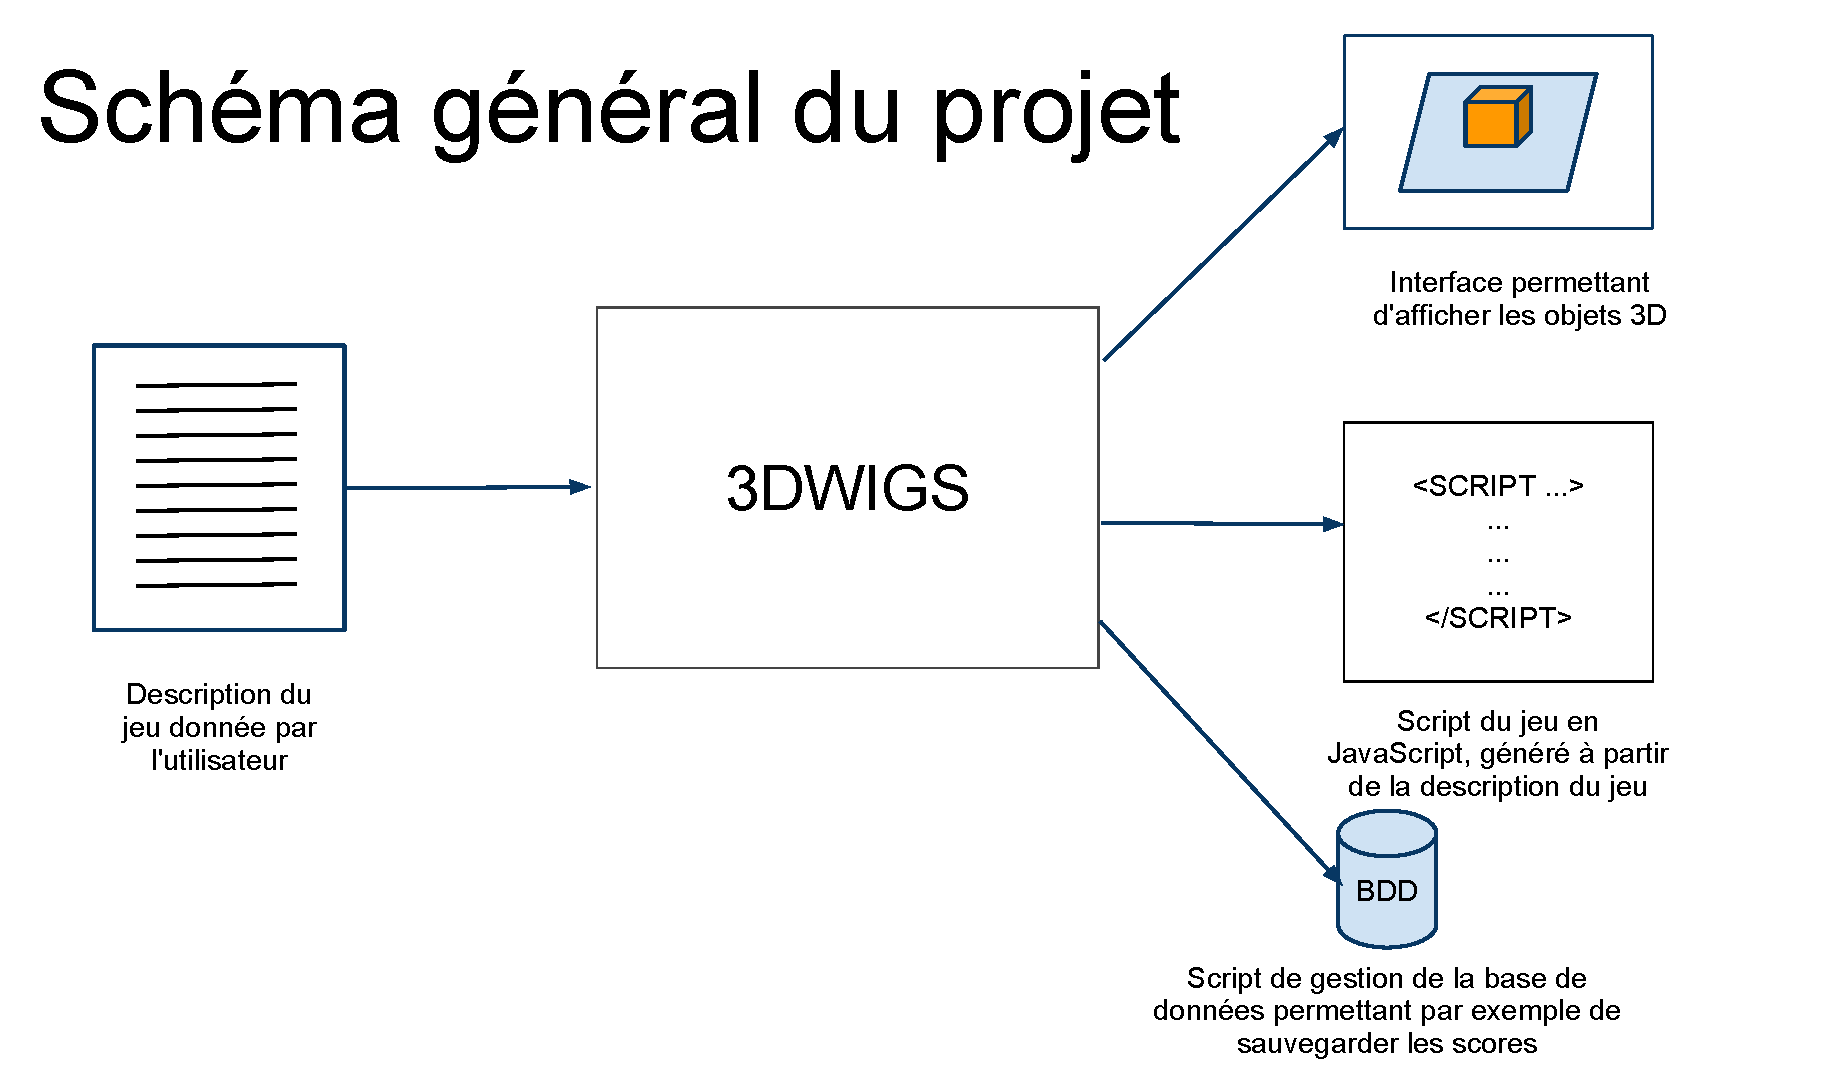
\includegraphics[height=7cm]{img/schema_general}
 \label{fig:schemaprojet}
\end{figure}

Le schéma général du projet est présenté sur la figure ci-dessus.
La partie gauche représente un fichier écrit par l'utilisateur contenant les règles du jeu qu'il souhaite créer respectant
une certaine syntaxe qu'il faut définir.

Il s'agit de créer un langage, à la fois suffisamment abstrait pour être accessible à n'importe quel utilisateur, mais également suffisamment riche
pour pouvoir décrire un maximum de jeux.
Le langage est défini par une grammaire.
Cette dernière doit permettre de décrire à la fois :
\begin{itemize}
 \item les objectifs ;
 \item les règles ;
 \item le scénario, les niveaux, la logique de score ;
 \item les interactions avec le(s) joueur(s).
\end{itemize}

Le challenge est difficile car il existe de très nombreuses catégories de jeux : 
par exemple, un jeu de gestion n'a, à première vue, aucun point commun avec un jeu de volley ou un jeu de plateforme.

Il serait illusoire de vouloir décrire absolument tous les jeux à l'aide d'une seule et unique grammaire.
En effet, les jeux décrits par une grammaire sont forcément restreints.

Toutefois, de nombreuses similarités existent entre plusieurs jeux. Il s'agit donc de les exploiter afin de définir un langage général de description de jeux.

Le fichier définissant le jeu via la grammaire se fera à l'aide d'un éditeur spécial, par exemple créé via eclipse.

\vspace{0.5cm}

La partie centrale du schéma correspond à un compilateur.
Il permet de convertir le fichier de description du jeu en un script javascript exécutable dans une page Web et permettant de jouer et 
interagir avec l'environnement.
Le langage javascript a été choisi pour la génération du jeu car il est actuellement le plus utilisé pour les interactions dans les pages Web.

La création et l'édition des objets 3D se fera à l'aide d'outils déjà très complets tel que Google SketchUp.
Leur affichage sera géré par WebGL.
\note{compléter un peu la partie 3D, dire ce qu'est WebGL tout ca peut être ?}

\vspace{0.5cm}

Dans un premier temps, des exemples classiques de mini-jeux seront présentés et analysés afin de mieux identifier
les différences et points communs entre différents types de jeux. Cette analyse mettra en évidence des notions classiques
présentes dans plusieurs jeux.
Dans une seconde partie, les concepts récurrents vus dans l'analyse et présents dans les grammaires seront détaillés.
Enfin, les langages proposés pour la description des jeux seront exposés en mettant en évidence leurs possibilités et leurs limites. 

\section{Les mini-jeux}
\label{sec:minijeux}
Le contenu des mini-jeux peut être très varié : jeu de rôle, jeu de gestion, jeu de plateforme, etc.
L'analyse des différences et des ressemblances entre ceux-ci, afin de définir ensuite une grammaire de description de jeux, est d'autant plus complexe.

Afin de nous confronter aux problèmes liés à l'implémentation de petits jeux vidéos et de faciliter l'analyse de la façon de décire un jeu, 
nous avons développé un échantillon de 8 types de mini-jeux en 2D dans le langage javascript.

Ces jeux n'ont pas été choisi par hasard : chacun possède un intérêt dans la description de ses règles et son implémentation.

\vspace{0.5cm}

\begin{tabular}{l|l}
 Jeu & Intérêt majeur \\
 \hline
 Pacman & ?? \\
 1942 & Vague d'ennemis \\
 Volley & Logique de score \\
 Course & Intelligence artificielle \\
 Mario & Niveaux \\
 Game\&Watch & ?? \\
 Billard & Collisions \\
 Jeu de Gestion & Ressources \\
\end{tabular}

\vspace{0.5cm}

Nous allons désormais présenter chacun de ces mini-jeux, pour ensuite analyser leurs objectifs, 
leurs règles et de façon plus générale leurs contenus afin d'en resortir différents aspects récurrents.

\subsection{Présentation des mini-jeux}

\note{c'est pour l'instant un bête copier coller de chacun, les fautes n'ont pas été corrigés.
On retravaillera cette sous-partie pour homogénéiser les différentes descriptions}

\subsubsection{Pacman}

Ce jeu est une adaptation du jeu classique de Pacman. 
Le joueur contrôle le TUX via les touches du clavier. 
Son but est de manger toutes les pommes sur le terrain tout en évitant les Microsoft qui essayent de l’attraper. 
Pour arriver a cet objectif, le joueur disposera de 3 vies. Le TUX pourra manger des pommes en or pour pouvoir détruire les Microsoft 
un petit temps et marquer quelques points en plus. En ce qui concerne l’affichage, le joueur verra le nombre de vie restante, 
son score ainsi que le temps ou les Microsoft restent vulnérables. Le Jeu est adaptable car il est facile d’initialiser 
la carte a partir d’images et d’un fichier Json.

\begin{figure}
 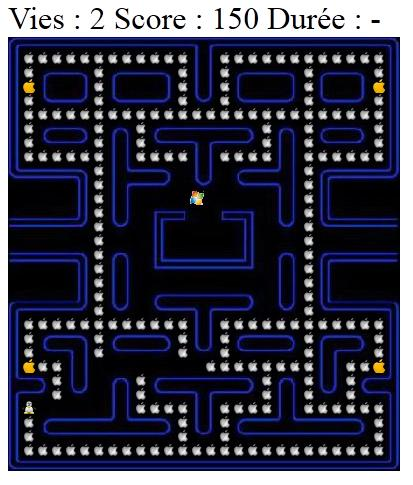
\includegraphics[width=\linewidth]{img/capturejeu_pacman}
 \caption{Capture du mini-jeu Pacman}
 \label{fig:game_pacman}
\end{figure}

\subsubsection{1942}

Dans ce shoot them up (jeu d’action où le joueur fait face à une multitude d’ennemis), 
le joueur contrôlera un vaisseau armé de deux canons pour détruire tous les véhicules adverses pour gagner des points. 
Le joueur aura 3 vies pour faire un maximum de point. Lorsque le joueur perd une vie, il devient invincible un petit moment pour reprendre la main ! 
Le vaisseau sera contrôlable via le clavier. En ce qui concerne les ennemis, ils suivent des déplacements prédéfinis qui peuvent être paramétrés. 
Le joueur n’est pas obligé de faire tuer tous les ennemis mais le but est quand même de faire le plus grand score !

\begin{figure}
 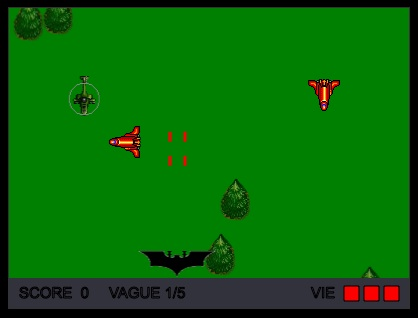
\includegraphics[width=\linewidth]{img/capturejeu_1942}
 \caption{Capture du mini-jeu 1942}
 \label{fig:game_1942}
\end{figure}

\subsubsection{Volley}


CowCow volley party  est un mini jeu humoristique mettant en scène deux vaches jouant au volley.
On peut jouer à ce jeu en mode solo avec une IA ou en multijoueur. 
Le but étant bien sur de gagner la partie en ayant 2 sets gagnants en premier. 
Pour cela votre vache dispose de 3 coups différents : passe courte et longue ainsi que le fameux smash !
Les règles de ce jeu sont les mêmes que les règles du volley classique. La vache sera contrôlée au clavier aussi bien  en mode multi qu’en mode solo.

\begin{figure}
 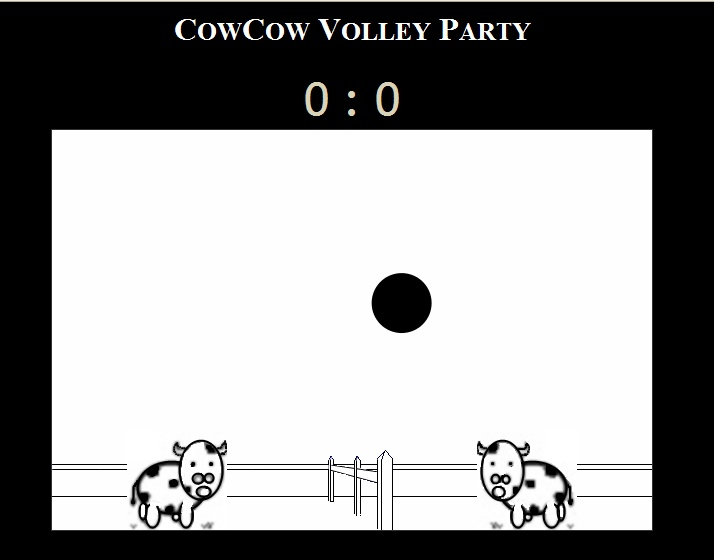
\includegraphics[width=\linewidth]{img/capturejeu_volleycowcow}
 \caption{Capture du mini-jeu volley}
 \label{fig:game_volley}
\end{figure}

\subsubsection{Course}

Ce jeu de course futuriste pour le web est un jeu pour un joueur qui se frottera à des intelligences artificielles pour faire le meilleur temps. 
Ce jeu de courses n’est pas un jeu de course classique, en effet sur le circuit vous trouverez des bonus 
(un turbo, un bonus permettant d’augmenter le temps d’un des autres joueurs, de changer leur positions, etc) 
et des zones de circuit différentes (inversion des commandes sur une zone, changement de vitesses, etc) 
ainsi que des objets fixes (turbo au sol,…). Vous pourrez choisir votre véhicule parmi une sélection de 12 vaisseaux différents. 
 En ce qui concerne les contrôles, le joueur se dirigera grâce à son clavier. Ce jeu est adaptable, il est, en effet, 
possible de créer facilement des circuits ainsi que des nouveaux bonus. Il serait aussi possible de mettre en place un système de 
lecture de fichier pour configurer les paramètres des différentes courses.

\begin{figure}
 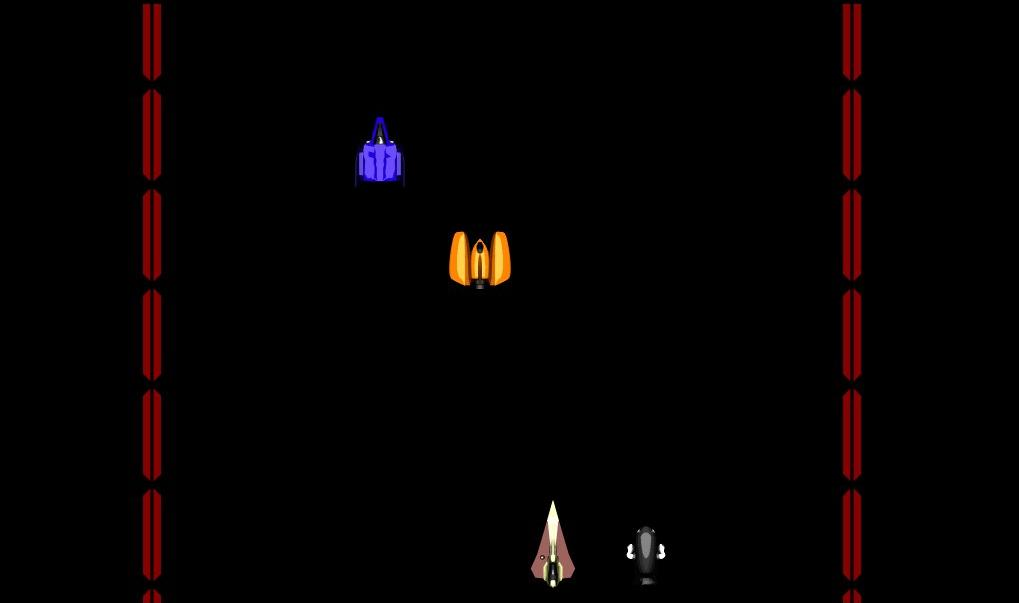
\includegraphics[width=\linewidth]{img/capturejeu_course}
 \caption{Capture du mini-jeu de course}
 \label{fig:game_course}
\end{figure}

\subsubsection{Mario}

Ce mini-jeu de plateforme reprend le principe des jeux du style de mario bros.
Un personnage, représenté par un rectangle, peut se déplacer sur les côtés ou sauter.
Il doit avancer au maximum, sans être touché par des ennemis, représentés par des triangles et sans tomber dans les trous du terrain.
Le personnage peut faire perdre des points de vie aux ennemis jusqu'à les tuer en leur sautant dessus. S'il les touche sur les côté, 
il meurt et la partie est terminée.
La caméra avance lorsque le joueur avance suffisamment. Le joueur peut revenir à gauche jusqu'à la limite de l'écran.
Le terrain est généré aléatoirement et est infini.
Le but du jeu est d'obtenir le plus grand score. Le score diminue avec le temps et augmente lorsqu'un ennemi est tué ou que le personnage avance

\subsubsection{Game \& Watch}

L’application est un mini-jeu du style Game \& Watch, où le personnage principal doit chasser ses ennemis avant que ces derniers ne l’atteignent.

Lors du jeu, les ennemis arrivent du bas de l’écran, et montent jusqu’à arriver au niveau du personnage, qui doit les écraser. S’il ne le fait pas, 
il perd une vie. A 0 vie, le jeu s’arrête et le joueur perd la partie.

Pour chaque ennemi écrasé, le joueur gagne un point déterminé de point. A partir d’un certain nombre de points qui sera définit plus tard, 
le jeu passe au niveau suivant, ce qui se traduit par l’augmentation de la difficulté, c’est-à-dire l’arrivée des ennemis s’accélère.

Lorsque le joueur arrive à détruire un de ses ennemis, il gagne un certains nombre de points. Par contre, lorsqu’un ennemi atteint le joueur, 
ce dernier perd une vie et son score reste intact.

Quand le joueur perd la partie, il doit pouvoir sauvegarder son score si ce dernier est dans les 5 meilleurs scores et si le joueur le souhaite.

Lorsqu’il ne reste au joueur que 2 vies, des vies “bonus” apparaissent pendant un certain temps, une à une, puis disparaissent; 
le joueur doit donc se déplacer vers elles pour les récupérer et augmenter ainsi son niveau de vie.

Les ennemis arrivent un par un du bas vers le haut, où se situe le joueur. 
La vitesse à laquelle ces ennemis arrivent est déterminée par le niveau actuel du jeu. 
Plus les niveaux augmentent plus la vitesse des ennemis s’accélère.

\begin{figure}
 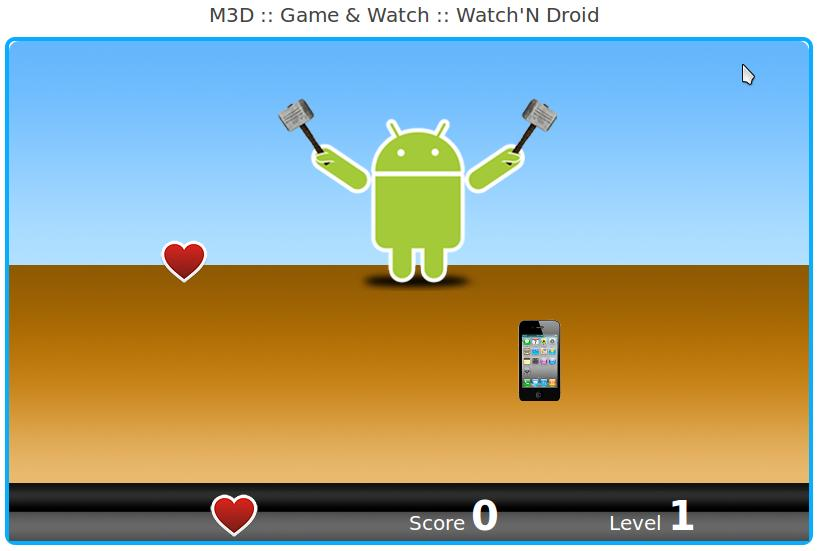
\includegraphics[width=\linewidth]{img/capturejeu_watchndroid}
 \caption{Capture du mini-jeu Game \& Watch}
 \label{fig:game_gamewatch}
\end{figure}

\subsubsection{Billard}

Ce mini-jeu de billard est un jeu multi-joueurs au tour par tour. 
Il reprend les règles classiques du billard anglais (chaque joueur doit rentrer toutes les boules d’une couleur puis la noire). 
D’un point de vue gameplay, le joueur contrôle la queue qui pointe automatiquement vers la boule blanche via sa souris. 
Le joueur peut ainsi choisir l’angle avec lequel il compte frapper la boule blanche et en fonction du pendant lequel le joueur va cliquer le tir va être plus ou moins fort. 
Pour l’affichage, chaque joueur voit combien de boules sont rentrés ainsi que sa couleur. Une icône verte apparait au niveau du joueur qui doit jouer. 
Le cadre bleu en bas de l’écran affiche la personne ayant gagné la partie !

\begin{figure}
 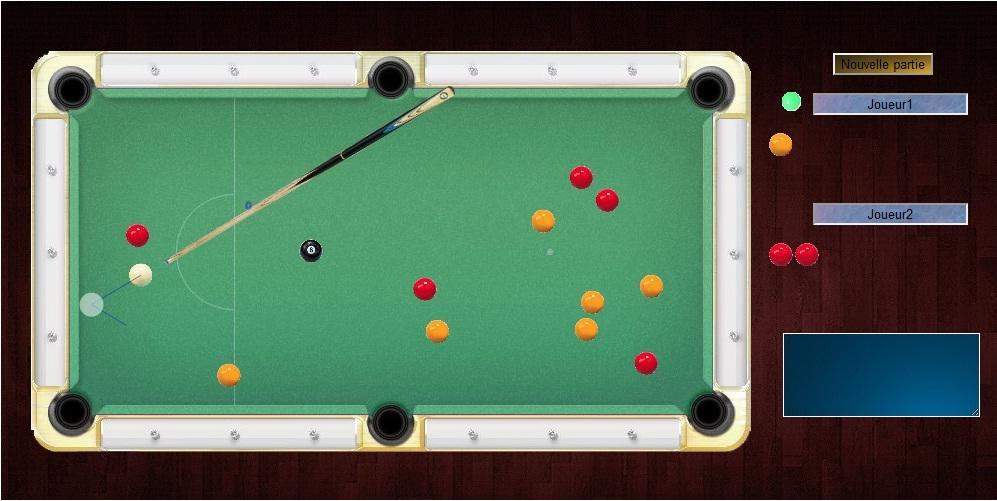
\includegraphics[width=\linewidth]{img/capturejeu_billard}
 \caption{Capture du mini-jeu billard}
 \label{fig:game_billard}
\end{figure}

\subsubsection{Gestion}

Le jeu commissariat est  un jeu de gestion du style Farmville. 
Vous aurez pour rôle de maintenir et améliorer votre commissariat en fonction des ressources disponibles.
 Les ressources sont au nombre de quatre : le nombre de policier, l’argent, l’indice IGPN et l’alcool ! 
Il y a trois actions disponibles pour le joueur. Il peut envoyer des policiers en missions dans un quartier 
choisis pour ramener de l’argent ainsi qu’un prisonnier.  Si un prisonnier est ramené, le joueur a la possibilité 
de libérer le prisonnier contre de l’argent ou de le tabasser (avec un fort risque de pénalité). 
Il peut aussi acheter des équipements ainsi que de l’alcool avec son argent. L’alcool est une ressource qui diminue constamment, 
le joueur doit ton veiller a toujours en avoir pour ne pas perdre. Il peut aussi perdre avec un indice d’IGPN trop élevé, cet indice 
monte avec toutes les mauvaises actions (tabasser un prisonnier, etc.).

\begin{figure}
 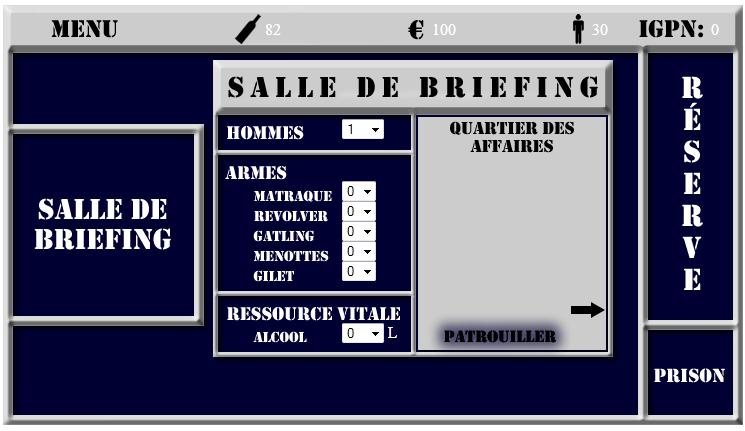
\includegraphics[width=\linewidth]{img/capturejeu_gestion2}
 \caption{Capture du mini-jeu de gestion}
 \label{fig:game_gestion}
\end{figure}

\subsection{Analyse des mini-jeux}

Suite au développement de ces mini-jeux, nous avons voulu analyser le contenu de ces différents jeux.
Pour cela, le tableau suivant récapitule différents aspects des jeux.

\note{inclure le tableau de google docs, en renvoyant peut être les colonnes pour mieux l'adapter à ce qu'on a fait dans la grammaire}

\vspace{0.5cm}

\begin{tabular}{|l|l}
\hline
 Jeu &   \\
\hline
 Pacman &  \\
\hline
 1942 &   \\
\hline
 Volley &  \\
\hline
 Course &  \\
\hline
 Mario &  \\
\hline
 Game\&Watch & \\
\hline
 Billard &  \\
\hline
 Jeu de Gestion & \\
\hline
\end{tabular}

\vspace{0.5cm}

Ce tableau permet de mieux identifier les différences et points communs entre les différents jeux.

On y voit par exemple que les objectifs au cours d'un niveau (ou pour un jeu sans niveau) revient souvent à atteindre une certaine zone
appelée ligne d'arrivée, ou éventuellement remplir des conditions de temps ou de ressources. En effet, à la fois la vie et le score
peuvent être vus comme une ressource : il s'agit d'un état, et une condition sur celui-ci est nécessaire à la victoire.
En faisant des conjonctions et des disjonctions de ces différentes possiblités, il est possible de définir 
les conditions de victoire pour tous les jeux (sauf le jeu de gestion).

En revanche, si on regarde comment le monde est construit, il est très différent d'un jeu à l'autre.
Pour certains comme Pacman, il est défini par une grille, pour d'autres comme le jeu de course, il est défini via un anneau.

Le tableau nous permet de voir assez clairement que le jeu de gestion est très différent des autres jeux.
Nous avons donc décidé de ne pas prendre en compte ce type de jeux.
Nous allons donc essayé de tirer des points communs entre les autres jeux, pour définir des concepts qui seront détaillés dans 
les parties suivantes.
Retirer de notre grammaire les jeux de gestion n'empêchent pas de couvrir un nombre important de jeux.
Il serait possible par exemple de définir plusieurs grammaires, chacune couvrant une catégorie de jeux afin de pouvoir
créer plusieurs types de jeux. Ainsi on pourrait créer une autre grammaire spécialement pour les jeux de gestion.
De la même façon, il est difficile de trouver des points communs entre les 7 mini-jeux restants, et un jeu de rôle où par exemple le joueur
doit réaliser plusieurs quetes.
Cependant, nous nous sommes concentrés pour le moment sur une unique grammaire décrivrant les 7 mini-jeux.

\note{Lister les concepts trouvés}


\section{Définition de concepts}
\label{sec:concept}
Certains concepts se trouvent dans beaucoup de mini-jeux. Le but est ici de les définir de manière précise.

\subsection*{Définition générale d'un jeu}

\underline{Jeu} : 
Activité de loisir soumise à des règles et ayant des objectifs (à la différence d'un jouet). Il s'agit ici d'un contenu numérique
 disponible via un site internet.

\underline{Règles du jeu} : 
Ensemble de principes qui décrivent le fonctionnement du jeu et 
la façon dont les éléments qui le composent interagissent entre eux. 
Ces règles définissent également les conditions nécessaires à la victoire (objectifs).

\subsection*{Element d'un jeu}

\underline{Environnement} : 
Univers du jeu. 
Plus précisément, il s'agit des décors qui le composent, des entités et des objets qui s'y trouvent ainsi que 
des règles physiques qui s'y appliquent comme la gravitation.

\underline{Terrain} : 
Socle de l'environnement.

\underline{Entité} : 
Elément animé présent dans l'environnement ou pouvant changer d'état. 
Elle dispose de caractéristiques et d'un panel d'actions prédéfinies qui lui sont propres.

\underline{Décor} : 
Elément inerte présent dans l'environnement.


\subsection*{Titre à trouver x)}

\underline{Ressource} : 
Elément virtuel d'un jeu exprimé sous forme numérique, pouvannt servir de monnaie, de matière première, d'état, etc.

\underline{Inventaire} : 
Ensemble des objets dont dispose une entité et qu'elle transporte avec elle.

\underline{Vie} : 
Ressource particulière associée aux entités mortelles et aux objets destructibles du jeu.


\subsection*{Contrôle direct/indirect}

\underline{Contrôle direct} :
Capacité du joueur à interagir sur l’environnement limitée à une seule entité à un instant t. 
Les actions dont il dispose sont celles dont l'entité dispose.

\underline{Contrôle indirect} :
Capacité du joueur à interagir sur l’environnement plus complexe. 
Les actions dont il dispose sont définies à la création du jeu et ne se limite pas au contrôle et aux actions d'une unique entité.

\subsection*{Environnement linéaire/non linéaie}

\underline{Environnement linéaire} : 
Environnement dans lequel le joueur doit suivre un cheminement prédéfini. (ex: Tomb Raider).

\underline{Environnement non linéaire} : 
Environnement dans lequel le joueur est libre d'évoluer comme il le souhaite. 
Il n'y a donc pas d'obligation à accomplir les objectifs dans un ordre précis.


\subsection*{Autre ...}

\underline{Niveau} :

\underline{Allié,ennemi,neutre} :

\underline{Entité réactive/autonome}



\section{Grammaires}
\label{sec:grammaire}
Trouver une grammaire riche, complète et accessible à n'importe quel utilisateur est difficile.
C'est pourquoi, en réalité deux grammaires sont présentées.

\begin{itemize}
 \item La première est dite de 'haut-niveau'.
Elle permet de décrire la majorité du contenu du jeu dans un langage simple de compréhension.
 \item La seconde est dite de 'bas-niveau'.
Elle permet de manipuler chaque attribut et est beaucoup plus proche de l'implémentation finale que la première grammaire.
C'est par exemple elle qui permettra de définir le comportement de l'intelligence artificielle, chose très difficile à mettre en oeurvre à haut-niveau.
\end{itemize}

Le schéma de compilation se complexifie alors : un fichier décrivant le jeu dans la grammaire de haut-niveau est compilé afin de donner un fichier
respectant la grammaire de bas-niveau. A ce niveau là, l'utilisateur peut effectuer de nouveaux ajouts ou modifications. Le second compilateur
produit alors le script final du jeu en javascript.

\subsection{Grammaire haut-niveau}

La description du jeu se déroule en plusieurs phases.
Elle commence par les entités du jeu : personnage, ennemis, alliés et leurs attributs.
Viennent ensuite les définitions d'actions de base et des commandes.
Enfin, les règles du jeu sont spécifiées.

\subsubsection{Définition des entités du jeu et de leurs attributs}

Il s'agit de lister les différents personnages ou objets qui apparaissent dans le jeu.
Pour faciliter le travail de l'utilisateur, diverses classes sont déjà créées pour définir les entités.
La classe de base est la classe Object avec des attributs de base comme la position, l'orientation, la taille, etc.
De celle-ci héritent de nombreuses autres classes comme Character, Vehicle ou Weapon chacun ayant des nouveaux attributs spécifiques.
\note{Inclure le schéma des classes ?}

La déclaration d'un nouveau personnage se fait alors via un identificateur et le mot-clef 'is'.
Par exemple \code{Mario is Character} permet de déclarer Mario comme un personnage de classe Character, 
et peut donc posséder tous les attributs de cette classe. Ces derniers sont initialisés à des valeurs par défaut.
Pour modifier cette initialisation, par exemple pour changer l'attribut \code{lifeMax} de Mario, les mots clefs 'has' et 'at' sont utilisés : 
\code{Mario has lifeMax at 3}.
De même, il est nécessaire de pouvoir rajouter de nouveaux attributs à Mario.
La syntaxe est la même. Ainsi, \code{Mario has energie at 8} ajoute un attribut énergie à Mario, initialisé à 8.
Les nouveaux attributs doivent obligatoirement être initialisés grâce à 'at'.

De plus, s'il existe divers personnages qui possèdent aussi cette énergie, il est souhaitable de ne pas avoir à répéter cette ligne.
Ainsi, de nouveaux types peuvent être crées grâce au mot-clef 'type' :
\code{type Plombier is Character. Plombier has energie at 8. Mario is Plombier. Luigi is Plombier.}
\note{a-t'on l'héritage multiple et si oui, comment ce la se passe en cas d'attributs du même nom ?}

Ensuite, en même temps que la déclaration de la classe d'une nouvelle identité, il est possible de la définir comme jouée par le joueur, ennemi, allié ou neutre.
(Si cela n'est pas précisé, la valeur est mise à neutre par défaut.
\code{Mario is Plombier player. Luigi is Plombier ally. type Boss is Character ennemy. Bowser is Boss.}
De plus, dans le cas où ce n'est pas un personnage joué, il peut être déclaré comme multiple.
Cela signifie qu'il est possible d'en générer plusieurs avec la seule commande 'generate'.
Par exemple \code{Koopa is} \code{Character enemy multiple. generate 5 Koopa in zone}. Permet de créer 5 Koopa dans \code{zone} qui aura dû être définie
auparavant. Outre 'in', les mots-clefs 'on' permet de placer des objets juste au-dessus de la zone définie par le mot suivant, et le mot-clef 'at' génère
le premier objet à l'endroit indiqué et les autres proches de celui-ci, tout en évitant les collisions.
\note{A confirmer que ce soit ça pour multiple}

Enfin, il est possible de manipuler des listes de ces classes.
\begin{lstlisting}[language=GameGrammar]
type humain is Character. 
type elfe is Character. 
type nain is Character. 
type hobbit is Character. 
type magicien is Character. 
gandalf is magicien ally.
CommunauteDeLAnneau is list of 1 elfe with 1 nain with 2 humain with gandalf with 4 hobbit.}
\end{lstlisting}

\subsubsection{Autres classes prédéfinies}

D'autres classes sont prédéfinies : une classe Game concernant l'ensemble général du jeu, une classe Camera contenant les informations sur les caméras :
certains comportements classiques sont prédéfinies comme un suivi à la première ou troisième personne, ou une caméra libre.

De plus, 2 clases permettent de gérer respectivement les compteurs et les ressources de type temporels.

\subsubsection{Définition de nouvelles actions et assignation des commandes}

Il est ensuite possible de définir de nouvelles actions via le mot-clef 'definition' et 'means'.
Par exemple, en reprenant l'exemple de Mario : \code{Mario is Character player. definition suicide means mario dies.}

Les commandes sont ensuite définies après le mot-clef 'command'. Elles sont générées soit par l'appui d'une touche X du clavier ('key X') soit par 
une action Y sur la souris ('mouse Y').
\code{command mouse rClick for suicide} permet par exemple de causer l'action nommée suicide lorsque le joueur clique sur le bouton droit de la souris.

De plus, de nombreuses actions sont prédéfinies pour les personnes du jeu comme jump ou move left ou concernant le jeu en général comme pause, save ou gameover.
\code{command mario is key space for jump,} \code{ key Z for move forward, key Y for move backward, key S for move left, key D for move right.}

Il est possible de désactiver (respectivement d'activer) certaines touches du clavier ou action de la souris au cours du jeu.
Pour cela, il faut utiliser le mot-clef 'desactive' (respectivement 'activate').
\code{desactive key Z} désactive les actions lors de l'appui sur la touche Z.
Il est également possible de désactiver toutes les commandes \code{desactive commands} ou toutes les commandes claviers \code{desactive key}.

\subsubsection{Déclaration des règles du jeu}

Les règles du jeu sont définies par le mot-clef 'rule' et 'then'.
Par exemple \code{rule mario dies then gameover}.

Il est également possible de manipuler les attributs des différentes entités. Prenons le cas où un ennemi a été défini \code{bowser is Character ennemy}
et que si mario entre en collision avec lui , alors il perd un point de vie, réduit son score de 100 et provoque un saut.
\code{rule mario touches bowser then sub 1 for life of} \code{ mario, sub 100 for score of game, mario jump}.

Outre 'sub' d'autres mots clefs existent pour les autres opérations arithmétiques élémentaires, ainsi qu'un 'assign' qui change directement
la valeur de l'attribut.

Certains concepts sont déjà définies : ainsi 'touches' est causée par une entrée en collision entre les deux entités, dies signifient l'arrivée de l'attribut
life à 0, kills se produit lorsque le premier personnage tue le second.
\note{j'ai un peu de mal à voir tout comment marche les declencheur et les conséquences dans la grammaire, du coup, je veux bien que 
quelqu'un nous explique tout ca, il doit manquer pas mal de choses là encore.}

\subsubsection{Exemple de mini-jeu décrit dans la grammaire 'haut-niveau'}

\note{Nous pensions éventuellement à un simple jeu à caméra fixe avec terrain prédéfini ou le personnage doit éviter certains ennemis
et prendre toutes les pièces avant d'atteindre un point d'arrivée, en fait genre un pacman sans bonus quoi :p, parce que mario on a le problème
des collisions par le haut ou pas, ainsi que la génération du terrain}

\subsection{Grammaire bas-niveau}

La grammaire bas-niveau est beaucoup plus proche de l'implémentation finale que la haut-niveau.
Ainsi, toutes les ressources doivent avoir un identifiant unique, les évènements qu'ils proviennent du joueur (clavier, souris) ou de la moficiation
de l'état d'un personnage sont gérés par des signaux.
La description d'un jeu est constitué de ressources, d'entités, de caméra, d'une boucle de rafraîchissement, d'un gestionnaire d'évènements.
Un moteur physique permettant de tester les collisions et contenant également les forces générales du jeu (gravitation, vent, etc.) est également disponible.

\subsubsection{Définition des ressources}

Une ressource est une variable du jeu qui pourra ensuite être attribuée à une entité.
Elle est identifiée par un nom unique.

\code{marioLife 1} permet de créer une ressource marioLife initialisée à 1.

Il existe un type spécial de ressource : les ressources temporelles.
Celles-ci sont mises à jour via la boucle de rafraîchissement générale du jeu.
Pour la définir, cette fois 2 valeurs sont données suites à la ressource : le pas du timer, et sont initialisation :
\code{timeStarBonus 10000 0} permet de créer une ressource de nom 'timerStarBonus' (pouvant correspondre à la durée du bonus donné par une étoile)
avec un pas de 10 secondes, et initialisée à 0 milisecondes. 

Il est également possible de faire des énumérations de ressources.
\note{il faudrait un joli exemple}

\subsubsection{Définition des entités et caméras}

On considère que le terrain est représenté par exemple par une matrice de points dans l'espace surlaquelle est aplliquée une texture.
La matrice pourra être remplacée selon le type de terrain pour un certain jeu. \note{Ca veut un peut rien dire ça, non ?}

L'ensemble des entités d'un jeu est alors constitué d'un terrain et d'un ensemble d'objet.
Chaque objet est identifié par un nom, ainsi que par deux fichiers créés par des outils de dessin d'objets 3D, un fichier .obj contenant l'ensemble
des points de l'objet, et un ficier .mat contenant la texture appliquée sur les faces de l'objet.
De plus chaque objet contient un ensemble de paramètre comme la vitesse, la position, etc. \note{vérifier le format de sortie de Sketchup}

Les caméras sont définies de manière similaire aux entités : chaque caméra est définie par un nom, une position et une orientation.

\note{comment on associe des ressources à une entité ?}

\subsubsection{Boucle de rafraîchissement et gestionnaire d'évènements}

Les divers évènements du jeu sont gérés via un système de signaux.

Le jeu dispose d'une boucle de rafraîchissement principale. Celle-ci génère un signal
signalUpdateCounter émettant un signal régulièrement.
De même, il permet de vérifier les touches enfoncées et actions de la souris à chaque tic du timer.

Enfin, chaque mise à jour de ressource nommée X émet un signal updateX.

Les actions lors de la réception d'un signal sont gérées par un gestionnaire d'évènements.
Ce dernier est défini par un ensemble de signaux et d'instructions.
Les instructions sont données comme dans un langage classique.
Elles sont composées des mises à jours de variable en utilisant les opérateurs arithmétiques classiques, les constantes, les autres ressources et des nombres
aléatoires.
Des instructions conditionnelles sont également disponibles, les booléens étant générés via des comparaisons d'expressions.

Les instructions peuvent également reprendre des concepts classiques de mini-jeux : pause, nouvelle partie, fin de partie, sauvegarde de la partie.
\note{insérer un petit exemple}

\subsubsection{Exemple de mini-jeu dans la grammaire bas-niveau}

\note{to do ...}

\section{Stratégie de Développement}
\label{sec:strategie}

Cette partie présente la prévision du travail du second semestre. La figure ci-dessous montre le diagramme de Gantt du planning prévisionnel pour celui-ci.

\begin{figure}[h]
 \centering
 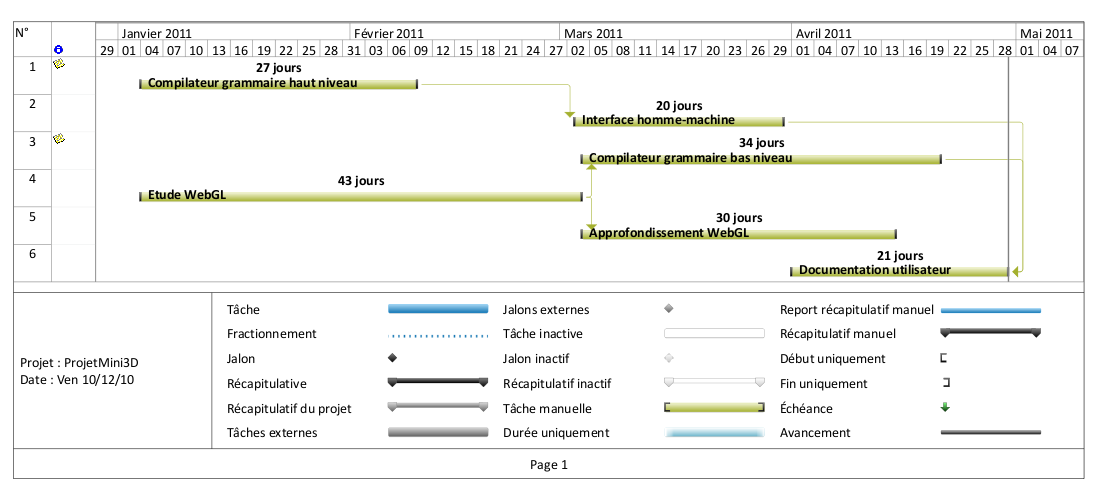
\includegraphics[width=\textwidth,height=6.5cm]{strategie/diag_gantt}
\end{figure}

La figure suivante est un descriptif des tâches planifiées et chemin critique.

\begin{figure}[h]
 \centering
 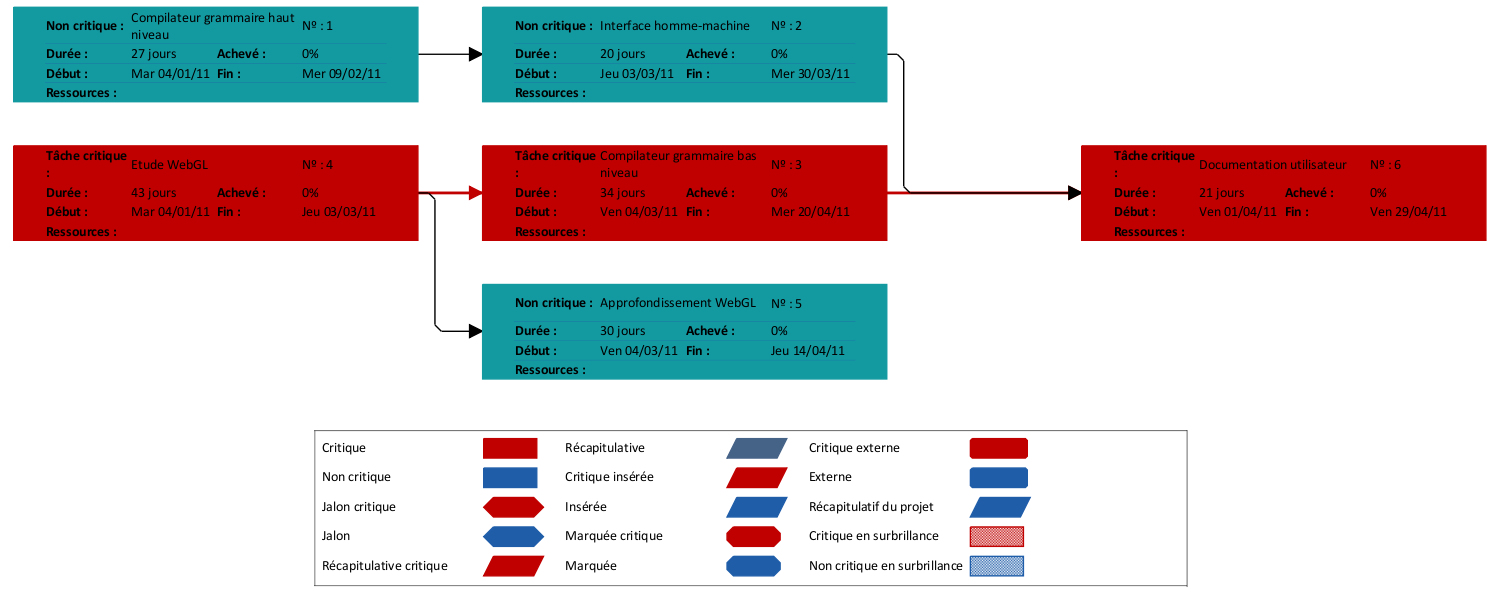
\includegraphics[width=\textwidth]{strategie/org_desc_tach}
\end{figure}

La première phase de développement se concentrera sur le compilateur du langage haut niveau qui ne nécessite pas d’apprentissage particulier 
puisque les bases du langage client (javascript) ont déjà été  étudiées lors de la phase d’analyse. 
En parallèle, sera effectuée une recherche générale sur l’utilisation de WebGL qui est un langage peu documenté car très récent, 
mais nécessaire à la suite du projet. Pour cette raison, une longue durée lui est consacrée.


WebGL incarne le principal risque du projet car nous ne savons pas le manipuler et nous ne connaissons pas ses limites.
 C’est une part d’inconnu qui pourrait potentiellement retarder le démarrage des tâches suivantes ainsi qu’affecter la bonne marche de celles 
liées au développement des compilateurs ; soit par obligation de modifier les grammaires établies pour répondre à des problèmes propres au WebGL 
soit par des difficultés d’implantation, causées par le manque de maturité du langage.

Une fois l’étude WebGL achevée, le développement du compilateur du langage bas niveau pourra commencer ainsi qu’un approfondissement de WebGL.


Lorsque les bases du compilateur du langage haut niveau seront établies, le développement de l’interface homme-machine pourra débuter.
 Un battement d’une semaine est prévu car il est fort probable que des modifications de ce compilateur aient lieu après une première finalisation.

La méthode agile répond aux besoins du projet, notamment à la souplesse qu’il demande. 
En conséquence, seront employés, le couple des méthodes Scrum et Extreme Programming. 

\appendix

\end{document}
